% This is "sig-alternate.tex" V2.0 May 2012
% This file should be compiled with V2.5 of "sig-alternate.cls" May 2012
%
% This example file demonstrates the use of the 'sig-alternate.cls'
% V2.5 LaTeX2e document class file. It is for those submitting
% articles to ACM Conference Proceedings WHO DO NOT WISH TO
% STRICTLY ADHERE TO THE SIGS (PUBS-BOARD-ENDORSED) STYLE.
% The 'sig-alternate.cls' file will produce a similar-looking,
% albeit, 'tighter' paper resulting in, invariably, fewer pages.
%
% ----------------------------------------------------------------------------------------------------------------
% This .tex file (and associated .cls V2.5) produces:
%       1) The Permission Statement
%       2) The Conference (location) Info information
%       3) The Copyright Line with ACM data
%       4) NO page numbers
%
% as against the acm_proc_article-sp.cls file which
% DOES NOT produce 1) thru' 3) above.
%
% Using 'sig-alternate.cls' you have control, however, from within
% the source .tex file, over both the CopyrightYear
% (defaulted to 200X) and the ACM Copyright Data
% (defaulted to X-XXXXX-XX-X/XX/XX).
% e.g.
% \CopyrightYear{2007} will cause 2007 to appear in the copyright line.
% \crdata{0-12345-67-8/90/12} will cause 0-12345-67-8/90/12 to appear in the copyright line.
%
% ---------------------------------------------------------------------------------------------------------------
% This .tex source is an example which *does* use
% the .bib file (from which the .bbl file % is produced).
% REMEMBER HOWEVER: After having produced the .bbl file,
% and prior to final submission, you *NEED* to 'insert'
% your .bbl file into your source .tex file so as to provide
% ONE 'self-contained' source file.
%
% ================= IF YOU HAVE QUESTIONS =======================
% Questions regarding the SIGS styles, SIGS policies and
% procedures, Conferences etc. should be sent to
% Adrienne Griscti (griscti@acm.org)
%
% Technical questions _only_ to
% Gerald Murray (murray@hq.acm.org)
% ===============================================================
%
% For tracking purposes - this is V2.0 - May 2012

\documentclass{sig-alternate}
\usepackage[T1]{fontenc}
\usepackage[utf8]{inputenc}
\usepackage{algorithm,caption,algpseudocode}
\usepackage[round]{natbib}
\usepackage{hyperref}

\newcommand\alert[1]{\textcolor{red}{#1}}
\newcommand\note[1]{\textcolor{blue}{#1}}
\newcommand\jb[1]{\textcolor{green!50!black}{#1}}

\begin{document}
%
% --- Author Metadata here ---
\conferenceinfo{ASSESS}{2014 New York City, USA}
%\CopyrightYear{2007} % Allows default copyright year (20XX) to be over-ridden - IF NEED BE.
%\crdata{0-12345-67-8/90/01}  % Allows default copyright data (0-89791-88-6/97/05) to be over-ridden - IF NEED BE.
% --- End of Author Metadata ---

\title{Item Response Theory vs. Q-Matrices for Adaptive Testing}
%\subtitle{An exhaustive survey}
%
% You need the command \numberofauthors to handle the 'placement
% and alignment' of the authors beneath the title.
%
% For aesthetic reasons, we recommend 'three authors at a time'
% i.e. three 'name/affiliation blocks' be placed beneath the title.
%
% NOTE: You are NOT restricted in how many 'rows' of
% "name/affiliations" may appear. We just ask that you restrict
% the number of 'columns' to three.
%
% Because of the available 'opening page real-estate'
% we ask you to refrain from putting more than six authors
% (two rows with three columns) beneath the article title.
% More than six makes the first-page appear very cluttered indeed.
%
% Use the \alignauthor commands to handle the names
% and affiliations for an 'aesthetic maximum' of six authors.
% Add names, affiliations, addresses for
% the seventh etc. author(s) as the argument for the
% \additionalauthors command.
% These 'additional authors' will be output/set for you
% without further effort on your part as the last section in
% the body of your article BEFORE References or any Appendices.

\numberofauthors{4} %  in this sample file, there are a *total*
% of EIGHT authors. SIX appear on the 'first-page' (for formatting
% reasons) and the remaining two appear in the \additionalauthors section.
%
\author{
% You can go ahead and credit any number of authors here,
% e.g. one 'row of three' or two rows (consisting of one row of three
% and a second row of one, two or three).
%
% The command \alignauthor (no curly braces needed) should
% precede each author name, affiliation/snail-mail address and
% e-mail address. Additionally, tag each line of
% affiliation/address with \affaddr, and tag the
% e-mail address with \email.
%
% 1st. author
\alignauthor \phantom{Jill-Jênn Vie}
       \affaddr{\phantom{ENS Cachan -- Bât. Cournot}}
       \affaddr{\phantom{61 av. du Président Wilson}}
       \affaddr{\phantom{94235 Cachan, France}}
       \email{\phantom{vie@jill-jenn.net}}
% 2nd. author
\alignauthor
\phantom{Fabrice Popineau}
       \affaddr{\phantom{Supélec -- Dép. informatique}}
       \affaddr{\phantom{3 rue Joliot Curie}}
       \affaddr{\phantom{91192 Gif-sur-Yvette, France}}
       \email{\phantom{fabrice.popineau@supelec.fr}}
% 3rd. author
\alignauthor
\phantom{Jean-Bastien Grill}
       \affaddr{\phantom{École normale supérieure}}
       \affaddr{\phantom{45 rue d'Ulm}}
       \affaddr{\phantom{75005 Paris}}
       \email{\phantom{grill@clipper.ens.fr}}
\and
% 4th. author
\alignauthor \phantom{Éric Bruillard}
       \affaddr{\phantom{ENS Cachan -- Bât. Cournot}}
       \affaddr{\phantom{61 av. du Président Wilson}}
       \affaddr{\phantom{94235 Cachan, France}}
       \email{\phantom{eric.bruillard@ens-cachan.fr}}
% 5th. author
\alignauthor
\phantom{Yolaine Bourda}
       \affaddr{\phantom{Supélec -- Dép. informatique}}
       \affaddr{\phantom{3 rue Joliot Curie}}
       \affaddr{\phantom{91192 Gif-sur-Yvette, France}}
       \email{\phantom{yolaine.bourda@supelec.fr}}
}
% There's nothing stopping you putting the seventh, eighth, etc.
% author on the opening page (as the 'third row') but we ask,
% for aesthetic reasons that you place these 'additional authors'
% in the \additional authors block, viz.
% \additionalauthors{Additional authors: John Smith (The Th{\o}rv{\"a}ld Group,
% email: {\texttt{jsmith@affiliation.org}}) and Julius P.~Kumquat
% (The Kumquat Consortium, email: {\texttt{jpkumquat@consortium.net}}).}
\date{June 24, 2014}
% Just remember to make sure that the TOTAL number of authors
% is the number that will appear on the first page PLUS the
% number that will appear in the \additionalauthors section.

\maketitle
\begin{abstract}
Computerized adaptive testing (CAT) is a mode of testing which has gained increasing popularity over the past years. It selects the questions asked to the examinee in order to evaluate her level efficiently, by using her answers to the previous questions.
Traditionally, CAT systems have been relying on item response theory (IRT) in order to provide an effective measure of latent abilities in possibly large-scale assessments.
More recently, from the perspective of providing useful feedback to examinees, other models have been studied for cognitive diagnosis. One of them is q-matrices, drawing a link between questions and examinee skills.
In this paper, we define a new framework to evaluate adaptive testing algorithms that enables us to use q-matrices in the context of assessments and to compare them to item response theory.
Our results suggest that q-matrices are better than IRT at predicting student answers.
\end{abstract}

% A category with the (minimum) three required fields
\category{}{Student assessment}{Adaptive testing}
%A category including the fourth, optional field follows...

\terms{Q-matrices, computerized adaptive testing, item response theory}

\keywords{Adaptive assessment, computerized adaptive testing, cognitive diagnosis, item response theory, q-matrices}

\newpage

\section{Introduction}
Automated assessment of student answers has recently gained popularity in the context of online initiatives such as the GMAT~\citep{Rudner2010}, or massive online open courses (MOOCs). Such systems must be able to rank thousands of students for evaluation or recruiting purposes and to provide personal feedback automatically in formative purposes.

If we already have a large-scale database of item responses for a certain test, it is natural to wonder which questions yield the most information about an examinee, i.e. if there is a ``best'' order in which the questions should be asked. In oral examinations, the examiner usually picks the next question to ask according to the previous answers of the examinee. Computerized adaptive testing (CAT) can be seen as an automated version of this process: keep asking the best possible questions until enough information has been gathered. Indeed, if the examinee behaves typically, a subset of carefully chosen results may be enough to guess how she will perform on the rest of the questions.

In order to fulfill this need, item response theory (IRT) is of great help. The initial purpose of IRT was to provide a framework to evaluate the performance of individual questions, called \emph{items}, on assessments~\citep{Hambleton1991}. It has been successfully applied to computerized adaptive testing and several methods have been proposed and implemented. According to her performance, an examinee gets a summative score, making it possible to predict her future answers. The simplicity of the IRT models both made it amenable to theoretical analysis~\citep{Baker2004} and further increased its popularity.

More recently, the No Child Left Behind Act of 2001 called for more formative assessments, putting emphasis on the early detection of students with cognitive disabilities and urged the need of cognitive diagnosis models. Instead of a summative score, examinees would receive a detailed feedback, specifying which skills are mastered and which ones are not~\citep{Cheng2009}. These models allow researchers to reveal possible misconceptions of the examinee in order to propose appropriate exercises. Most of these models rely on a q-matrix specifying for each question the different skills required to solve it. For example, a fraction test may require 1) converting a whole number to a fraction, 2) separating a whole number from a fraction, 3) simplifying before subtracting, and so on~\citep{DeLaTorreDouglas2004}. Cognitive diagnosis adaptive tests have been designed in order to guess the skills of the examinee effectively~\citep{Huebner2010}.

One could wonder why we compare a model designed for assessment with a model designed for feedback. We show that although q-matrices were first designed for formative assessments, it is also possible to use them in the context of large-scale assessments. Indeed, this model evaluates the skills of an examinee according to her previous answers. Given those computed skills and the q-matrix, we can predict her probability of correctly answering the remaining questions. This enables us to propose a framework for comparison that captures both models.

Originally, q-matrices were specified by experts, but recent work in the educational data mining field attempts to infer q-matrices directly from student data~\citep{Huebner2010}. The corresponding skills are therefore implicit, but such automatically extracted q-matrices have proven to produce better inference~\citep{Barnes2003}.

\subsection{Our contribution}

In this paper, we propose a new framework to evaluate adaptive testing algorithms and use it to compare the performances of both a traditional CAT using item response theory and a more recent cognitive diagnosis model from the literature in psychometrics using q-matrices. More precisely, we expect to answer the following question: given a budget of $B$ questions asked according to a certain adaptive selection rule, which model performs the best in predicting the answers of the examinee over the remaining questions? To the best of our knowledge, no such comparison has ever been made.

Whereas IRT is the most commonly used model for adaptive testing, q-matrices represent a good model for fine-grained cognitive diagnosis. In fact, our results show that the cognitive diagnosis model outperforms IRT.

\subsection{Outline}

We first present the computerized adaptive testing framework and two models chosen respectively from item response theory and cognitive diagnosis. We then detail the design of these models and the proposed framework to evaluate them in our simulation. Finally, we present our results.

\section{Background and Related Work}

\subsection{Computerized adaptive testing}

In a computerized adaptive test (CAT), the examinee is presented with adaptively selected questions according to her previous performance. Thus, a CAT framework relies on two main subroutines:
\begin{itemize}
\item \textsc{NextItem}: the item selection algorithm, that picks the next question to ask according to the previous answers of the examinee;
\item \textsc{TerminationRule}: a condition that will end the test, when enough information has been gathered and the competence has been measured satisfyingly.
\end{itemize}

The framework of a CAT can be represented by the following algorithm: while the termination rule is not satisfied, the algorithm picks the question that maximizes a certain criterion according to the item selection rule.

Common criteria for the item selection rule are minimizing the Shannon entropy of the distribution over the parameters, or maximizing the Kullback-Leibler divergence~\citep{Xu2003}.

\subsection{Item Response Theory}

For our needs, IRT provides a commonly used model allowing to compute the probability of answering correctly each question. Basically, IRT estimates the latent ability of a student by a unique real number $\theta$ modeled by a random variable and characterizes each question by two real numbers:

\begin{itemize}
\item the \emph{difficulty} $d$, corresponding to the ability needed to answer the question correctly;
\item the \emph{discrimination} $\delta$, representing the capacity of the question to draw a separation between students that have the required ability from those that do not.
\end{itemize}

Knowing the hidden ability $\theta_i$ of a given student $i$, the difficulty $d_j$ and the discrimination parameter $\delta_j$ of a given question $j$, the probability of the event ``the student $i$ answers correctly the question $j$'', which we denote by \emph{success}$_{ij}$, is modeled by:
\[ \Pr\{success_{ij}|\theta_i\} = \frac1{1+e^{-\delta_j(\theta_i - d_j)}}. \]

The aim is first to optimize the parameters $d_j$, $\delta_j$ for each question $j$ and $\theta_i$ for each student $i$ in order to fit a given train dataset. Then, during the CAT process, a probability distribution over $\theta_i$ is maintained and each question answered allows to refine the confidence interval around $\theta_i$ using the Bayes' rule. The probability of \emph{success}$_{ij}$ knowing the parameters can thus be computed by integrating over the hidden variable $\theta_i$.

\[ \Pr\{success_{ij}\} = \int \Pr\{success_{ij}|\theta_i\} \Pr\{\theta_i\} \mathrm d\theta_i \]

This simple model is used in computerized adaptive testing, where many methods are implemented for next item selection~\citep{MagisRaiche2012}.

\subsection{Cognitive Diagnosis Model}

The IRT model we just described uses a single parameter to represent students. We now develop a model that tries to be more informative about the student skills. Every student is modeled by a vector of binary values $(a_1, \ldots, a_K)$, called \emph{skill vector}, representing her mastery of $K$ different skills, thus leading to $2^K$ possible skill vectors. 

A q-matrix $Q$ \citep{Tatsuoka1983} represents the different skills involved in answering every question. Formally, $Q_{ij}$ is equal to 1 if the skill $j$ is involved in the resolution of question $i$, 0 otherwise. For example, in the following q-matrix, skills 1 and 2 are required to answer the first question, skills 1 and 3 are required for the second question and mastering skill 3 is sufficient to solve the last question.
\[ Q = \left(\begin{array}{lll}
1 & 1 & 0\\
1 & 0 & 1\\
0 & 0 & 1
\end{array}\right) \]
If all involved skills are necessary to succeed at corresponding item, the model is considered part of the \emph{conjunctive} class. 
If the mastery of one single skill is sufficient to succeed the item, it will be considered part of the \emph{compensatory} class. We consider here the NIDA model which is a conjunctive model~\citep{Desmarais2012} in presence of noise. More precisely, we denote by $s_i$ and $g_i$ the questions parameters, respectively called the \emph{slip} and \emph{guess} parameters of item $i$. The probability of a correct response at item $i$ is $1 - s_i$ if all skills involved are mastered, $g_i$ if any required skill is not mastered.

In the particular case $K=1$, the cognitive diagnostic model becomes close to the IRT model presented above, the only difference being the probability function of success. In the case of IRT, it defines a sigmoid, while in the q-matrix model for $K = 1$ it defines an affine function over $[0,1]$.

Determining the best q-matrix that fits a given student data set is currently an open field of research, as well as the most suitable number of attributes $K$~\citep{Huebner2010}, the state of the art being hill-climbing techniques~\citep{Barnes2005}, non-negative matrix factorization~\citep{Desmarais2011} or the EM algorithm~\citep{Huebner2010}. 

The skill vector of a student is a hidden variable modeled by a random variable. The number of different skill vectors being finite, it is possible to maintain the full probability distribution over the skill vectors and update it using Bayes' rule.

From this probability distribution over all possible skill vectors, with the help of our q-matrix, we can derive the probability for a given student to answer correctly any question of the test.

% Several methods for next item selection have been compared, such as Shannon entropy or Kullback-Leibler~\citep{Xu2003}. % TOUDOUX

%\begin{table} TODO
%\caption{Example for $K = 3$.}
%\end{table}

\section{Our Test Framework}

We now develop the different parts of the CAT process used in the simulation that will allow us to compare both presented models.

Our student data is a binary matrix of order $N_S \times N_Q$ where $N_S$ and $N_Q$ denote respectively the number of students and the number of questions, and $c_{ij}$ equals 1 if student $i$ answered the question $j$ correctly, 0 otherwise. 

We detail the cross-validation based method described in Algorithm 1. The dataset is partitioned into two sets, $train$ and $test$, \textsc{Simulate}$(train, test)$ trains our model on the $train$ dataset and evaluates it on the $test$ dataset.

\begin{itemize}
\item \textsc{TrainingStep}: Train the model in order to calibrate the question parameters $\alpha$. In the case of an IRT model, the difficulty $d_i$ and discrimination $\delta_i$ are computed for each question $i$, while in the case of cognitive diagnosis, the entries of the q-matrix $Q_{ij}$, the slip $s_i$ and guess $g_i$ are computed for each question $i$.
\item \textsc{PriorInitialization}: Initialize the prior $\pi$ on the student parameters, i.e. the distribution over the skills in the case of the q-matrix model and the distribution over the ability for the IRT model. 
\item \textsc{NextItem}: Choose the best question to ask according to a certain criterion given all previous questions and answers. 
\item \textsc{UpdateParameters}: Update the student parameters according to the previous answers.
\item \textsc{TerminationRule}: In our case, ``There have been $B$ questions asked so far.'' Indeed, as we want to compare different algorithms, we need to put them on an equal footing, i.e. ask the same number of questions in each case.
\item \textsc{PredictAnswers}: Compute the probability of correct answers of the student on the whole set of questions, i.e. compute for each question $i$ the probability for answering $i$ correctly.
\item \textsc{Evaluate}: Compare the true answers with the predicted ones in order to produce a performance indicator of the algorithm. 
\end{itemize}

\begin{algorithm}
\begin{algorithmic}
\Procedure{Simulate}{$train, test$}
\State $\alpha \gets \Call{TrainingStep}{train}$
\State $i \gets 0$
\For{all students $s$ in $test$}
	\State $\pi \gets \Call{PriorInitialization}$
	\While{\textsc{TerminationRule} is not satisfied}
		\State $q_{i + 1} \gets \Call{NextItem}{q_1, r_1, \ldots, q_i, r_i, \alpha, \pi}$
		\State Ask question $q_{i + 1}$ to the student $s$
		\State Get reply $r_{i + 1}$
		\State $\pi \gets \Call{EstimateParameters}{q_1, r_1, \ldots, q_i, r_i, \alpha}$
	\EndWhile
	\State $p \gets$ \Call{PredictPerformance}{$\alpha, \pi$}
	\State \Call{Evaluate}{$p$}
\EndFor
\EndProcedure
\end{algorithmic}
\caption{\textbf{CAT Framework}}
\end{algorithm}

\subsection{Logarithmic Error Function}

After having computed the probability of correct answers of the student, we need to compare them to the actual answers and deduce a performance indicator from it. For this purpose, we choose the popular logarithmic score~\citep{Gneiting2007}, that we will denote from now on by ``error''.

This quantity is both easy to define and to compute. Let $(p_i)$ be the probabilities of correct answer and $(a_i)$ be 1 if the answer was actually correct, 0 otherwise, the logarithmic score is then given by the following expression: 

\[ \sum_i a_i\ln(p_i) + (1-a_i)\ln(1-p_i).\]

\subsection{Item Response Theory Design}

This part of our experiments rely on an existing implementation of IRT. We still provide brief notes regarding their design. For more information, please consult \citep{Rizopoulos2006} and~\citep{MagisRaiche2012}.

\subsubsection{Training Step}

We compute for each question $j$ its difficulty $d_j$ along with its discrimination $\delta_j$ and also for each student $i$ her ability $\theta_i$ and the variance associated $v_i$ using the maximum likelihood estimator. Let $x_i$ be the unobserved true ability of student $i$, the log-likelihood can be expressed using the Bayes' formula. There are different ways of maximizing the log-likelihood, the chosen one being a variant of the EM algorithm.

\subsubsection{Item Selection Rule}

We pick at each step the question that maximizes the Fisher information. Similar results were obtained by minimizing the variance of the posterior distribution, but this method resulted in higher time complexity.

\subsubsection{Parameters Update}

After each student answer, we can recompute the posterior distribution over the student ability.

Sadly, for a normal or a logistic prior, the posterior distribution is no longer normal or logistic. Therefore, for an exact computation of the expectation and variance of the student ability, all the previous questions and answers are needed at each update.

\subsection{Cognitive Diagnosis Model Design}

\subsubsection{Training Step}

Within the psychometrics field, q-matrix are usually specified by experts, in order to get a feedback relying on intelligible skills. For our purpose, as q-matrices are a tool designed to predict the probability of a correct answer, we can learn this q-matrix from the data.

In order to extract a q-matrix achieving low likelihood, we need to estimate three kind of parameters: the binary entries of the q-matrix, the slip and guess parameters for each question, and a distribution of probabilities over all possible skill vectors for each student. Fixing any two, it is easy to optimize the third parameter, which suggests the following procedure: until convergence to a local minimum, sequentially optimize each parameter.

The estimation of the probability distribution over the skill vectors is done by Bayesian updates, asking all questions to each student. Also, the log likelihood can be expressed as a sum of convex functions of a single slip or guess parameter, therefore all slip and guess parameters can be independently and easily optimized.  Similarly, when the students skills, the slip and the guess parameters are fixed, the log-likelihood can be expressed as a sum of functions of a single q-matrix line. It follows that the optimization can be done line by line. In our case, the number of columns of the q-matrix is quite low, between 3 and 6 skills. Thus, there are at most $2^6 = 64$ possible lines and the best line can be found by simple exhaustive search.

%\alert{Cet algol converge vers un minimum local + minimum local peut être mauvais en particulier dans le cas K=6 (relancer depuis une autre matrice random)}

We would like to emphasize here that the purpose of this article is not to provide a more efficient algorithm for extracting q-matrices from real data. Nevertheless, our implementation is sufficient to provide results in a reasonable time. Indeed, we achieve a complexity of $O(N_Q N_S K 4^K)$ at each iteration where $N_Q$ and $N_S$ denote respectively the number of questions and the number of students, and $K$, the number of columns of the q-matrix, is at most 6 in our experiments.

\subsubsection{Item Selection Rule}

As an item selection rule, we choose the question minimizing the Shannon entropy of the distribution over the possible skill vectors.

\subsubsection{Parameters Update}

As the distribution over skills is on a finite support, we can maintain at each step the whole probability distribution $\pi$ over the possible skill vectors, initialized at the uniform distribution.
Knowing the student answer, the update of $\pi$ is done according to the Bayes' rule. Let $x$ be a skill vector, $s$ and $g$ the slip and guess parameters of a given question, if the skills associated to $x$ are sufficient to answer the question correctly,
\[ \pi_{n+1}(x) = \pi_n(x) \cdot [r\cdot(1-s) + (1-r)\cdot s] \]
otherwise
\[ \pi_{n+1}(x) = \pi_n(x) \cdot [r\cdot g + (1-r)\cdot(1-g)]. \]

\section{Evaluation}

\subsection{Data and Simulation Design} % and provided by Titus\footnote{\url{http://alumni.cs.ucr.edu/~titus/}}

We are using SAT Subject Test data, also featured in~\citep{Winters2005, Desmarais2011}. This student data is a $296 \times 40$ matrix representing the results from 296 students on 40 questions from the 4 following topics: Mathematics, Biology, World History and French.

In our experiments we analyze the effect of three parameters: the length of the training dataset, the number of questions of the test and the number of skills $K$ of the q-matrices. For both models considered, IRT and q-matrix, our test dataset was composed of the same 136 students, the last rows of the student data. The training dataset could be composed of the first 20, 40, 80 or 160 students, the number of questions of the test could be a random subset of 10, 20 or 40 questions picked from the dataset for each experiment. The number of skills of the q-matrix could be any integer from 3 to 6.

To evaluate the different models throughout the CAT process, we compute the mean error of the whole vector of predicted answers for all students of the test dataset, according to the ground truth.

Our implementation is written in Python and R using the packages \texttt{rpy2}~\citep{Gautier2008}, \texttt{ltm}~\citep{Rizopoulos2006} and\linebreak \texttt{catR}~\citep{MagisRaiche2012}. The code is available on Bitbucket\footnote{\url{http://bitbucket.org/no-suitable-for-blind-review/}}. The whole simulation process ran for 6 hours on a 1.3 GHz Intel Core i5.

\subsection{Results}

We compared the two presented algorithms, the IRT-based algorithm and our implementation of the NIDA q-matrix model for different values of the parameter $K$, the number of columns of the q-matrix.

We will first focus on the error of each algorithm after 10 questions for the 20-question test, for different sizes of the train dataset. Results are detailed in Table~\ref{tab:20q} where the best performances are shown in bold. As a reference, please note 0.693 is the error obtained by the trivial algorithm affecting every probability to 1/2. On the SAT dataset, for all reasonable choices of $K$, the q-matrix model outperforms IRT, the q-matrix of $K = 6$ skills being globally the best among all tested ones.

\begin{table}[H]
\small\centering\begin{tabular}{@{}cccc@{}}
$|train|$ & 40 & 80 & 160\\
\hline
IRT & 0.482 $\pm$ 0.022 & 0.473 $\pm$ 0.017 & 0.456 $\pm$ 0.019\\
Q $K = 3$ & 0.487 $\pm$ 0.016 & 0.470 $\pm$ 0.017 & 0.435 $\pm$ 0.012\\
Q $K = 4$ & \textbf{0.455 $\pm$ 0.017} & 0.434 $\pm$ 0.016 & 0.424 $\pm$ 0.016\\
Q $K = 5$ & 0.481 $\pm$ 0.022 & \textbf{0.399 $\pm$ 0.015} & 0.376 $\pm$ 0.013\\
Q $K = 6$ & \textbf{0.455 $\pm$ 0.023} & 0.400 $\pm$ 0.015 & \textbf{0.361 $\pm$ 0.015}\\
\end{tabular}
\caption{Mean error for a 20-question test, taken at mid-test.}
\label{tab:20q}
\end{table}

When the training set is composed of 160 students, IRT performs the worst among all tested algorithms, particularly when compared to the q-matrix model for $K = 6$. However, when the training set is composed of only 40 students, IRT performs slightly better than the q-matrix for $K = 3$. Also, the performance of the q-matrix for $K = 6$ improves drastically when the size of the training set increases, contrary to IRT or q-matrices with a low $K$ value.

For a deeper understanding, instead of computing the mean error only at mid-test, we compute it at each step of the CAT process for a train dataset of size 80 and a 20-question test. Results are shown in Figure~\ref{fig:1}. As we can see, IRT is not only performing the worst at mid-test but even in the early questions. Also, the greater $K$, the longer the corresponding q-matrix model takes to achieve its best performance.

We also computed the mean error of each algorithm after 20 questions of the 40-question test. Results are detailed in Table 2.

\begin{figure}
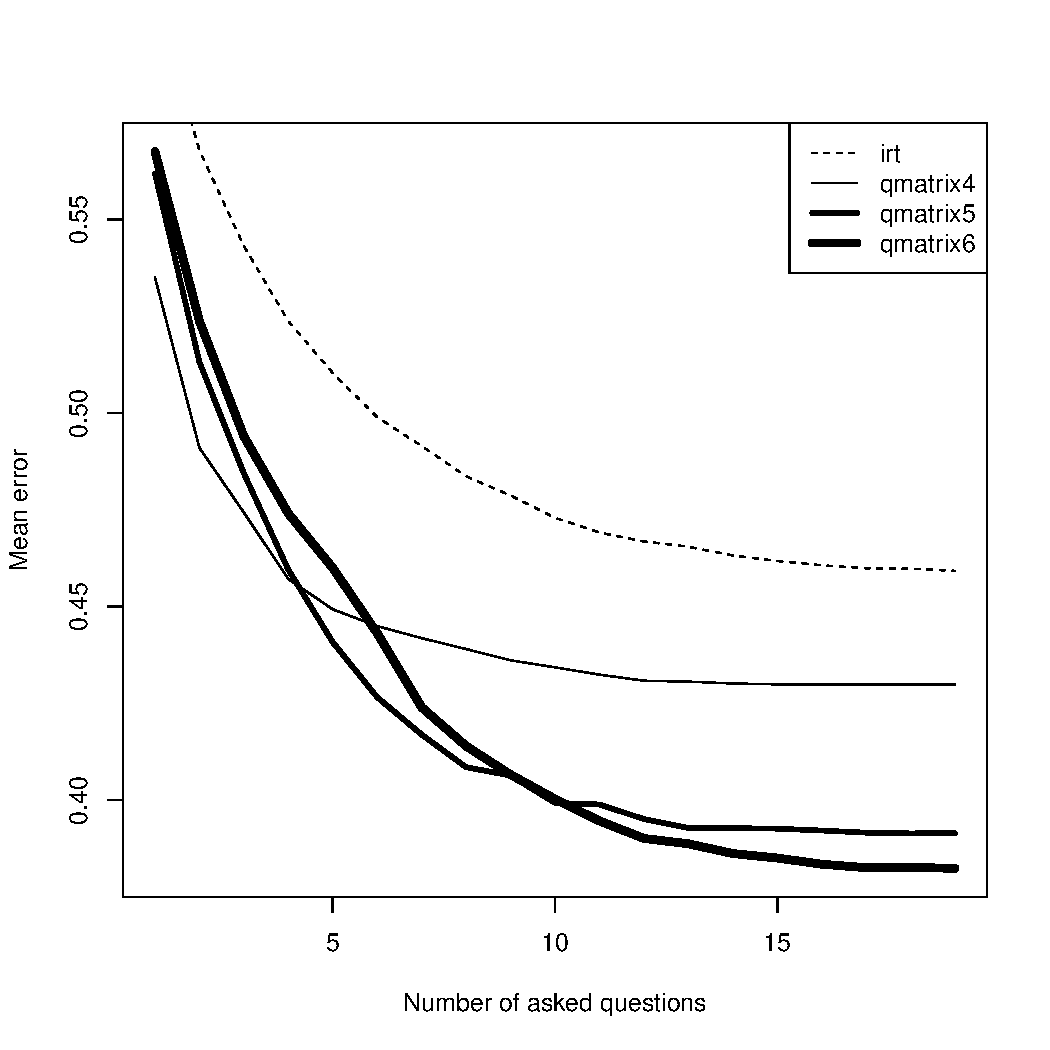
\includegraphics[width=\linewidth]{20-80.pdf}
\caption{Evolution of the mean error throughout the test, for a train dataset of size 80 and a 20-question test. The dashed curve denotes the IRT model, while the curves of growing thickness denote q-matrices of growing number of columns.}
\label{fig:1}
\end{figure}

\begin{table}[H]
\small\centering\begin{tabular}{@{}cccc@{}}
$|train|$ & 40 & 80 & 160\\
\hline
IRT & 0.499 $\pm$ 0.024 & 0.469 $\pm$ 0.020 & 0.446 $\pm$ 0.015\\
Q $K = 3$ & 0.517 $\pm$ 0.016 & 0.470 $\pm$ 0.012 & 0.444 $\pm$ 0.012\\
Q $K = 4$ & 0.494 $\pm$ 0.015 & 0.459 $\pm$ 0.011 & 0.417 $\pm$ 0.011\\
Q $K = 5$ & \textbf{0.474 $\pm$ 0.014} & 0.433 $\pm$ 0.011 & 0.415 $\pm$ 0.011\\
Q $K = 6$ & 0.482 $\pm$ 0.015 & \textbf{0.425 $\pm$ 0.012} & \textbf{0.403 $\pm$ 0.011}\\
\end{tabular}
\caption{Mean error for the whole 40-question test.}
\label{tab:40q}
\end{table}

\section{Discussion and Future Work}

Our studies suggest that the q-matrix model, first designed for cognitive diagnosis, can successfully be used in a context of assessments. Indeed, the fast and accurate estimation of the student skills enabled by our item selection induced a good prediction after few questions. This makes this model suitable for placement tests, where very few questions should be enough to explore at best the examinee's skills. More globally, it can be used for low-stakes testing, but not high-stakes testing, as the first questions chosen by the item selection rule are often the same. This high item exposure rate was already pointed out in~\citep{Cheng2009}.

Pay attention to the fact that although the training step is longer for the q-matrix model than the IRT chosen model, the next-item step is several times longer for the IRT model with minimum expected posterior variance criterion than the q-matrix model. Thus, for a given test, once a good q-matrix has been computed in a preprocessing step, the test can be administered in a reasonable time. % Can be linked to the prior.

However, q-matrix being a richer model, it can be prone to overfitting, particularly for greater values of $K$, as highlighted by our results. In addition, the longer convergence time for high values of $K$ can be explained by the fact that guessing a larger skill vector requires more information, therefore more questions. Thus, there is a tradeoff between a large value of $K$ potentially leading to overfitting and smaller ones which could not provide a rich enough model. The optimal value of $K$ may depend on the size of the training set along with the number of questions of the test. Nevertheless, as pointed out in~\citep{Huebner2010}, there have been no systematic studies for cognitive diagnosis models investigating the most suitable number of skills $K$ for a given dataset.

% Finally, while the optimization of the $K$ parameter is important, the sensibility of the results to this parameter is tempered. Indeed, the results for q-matrix with $K = 5$ and $K = 6$ are actually pretty close. % K

% Our results suggest that q-matrix is not very sensitive to the choice of K as long as this K parameters keep being reasonable given the train dataset.

Due to limited resources, our simulation was limited to $K \leqslant 6$. Indeed, the most costly part of the process is the training step of the q-matrix, which requires at each iteration a cost exponential in $K$ and a number of iterations increasing with $K$ to obtain convergence towards a local minimum. A better computation of q-matrix using more cutting-edge techniques could have lead to even better results.

%Our results can extended to other cognitive diagnosis models from the compensatory classes (DINA, etc.~\cite{Desmarais2011}).

%A new direction could be to 

%Please also note that, our item exposure rate is very high as the same first questions are asked. Thus low stakes high stakes

% On another note, our results are produced from a dataset over 4 knowledge fields. It would be interesting to compare IRT-based models and q-matrix models on other real data such as bigger datasets or ones including only one knowledge field.



We showed that links between questions are worth taking into account, something q-matrices do and IRT does not. For our evaluation, we chose the simplest models from item response theory and cognitive diagnosis, but more complex models such as multidimensional item response theory~\citep{Desmarais2012} or fusion models~\citep{McGlohen2008} should be compared to the NIDA q-matrix model presented here.

% MIRT

% As a finish we would like to draw a link between Elo systems and IRT because the probability of winning only depends on the difference between Elo values while the probability of answering correctly. 

% Chess stuff.

%Add a last column to q-matrix

%No study has been done yet over the number of skills.

%Outperforms on both simulated data and real data.

\section{Acknowledgements}

We thank \phantom{Chia-Tche Chang, Le Thanh Dung Nguyen and especially Antoine Amarilli} for their valuable comments.

%\bibliographystyle{abbrv}
\bibliographystyle{plainnat}
\bibliography{sigproc}  % sigproc.bib is the name of the Bibliography in this case
% You must have a proper ".bib" file
%  and remember to run:
% latex bibtex latex latex
% to resolve all references
%
% ACM needs 'a single self-contained file'!
%
%APPENDICES are optional
%\balancecolumns
%\appendix
%Appendix A
%\section{If I have something more to say}

%\balancecolumns % GM June 2007
% That's all folks!
\end{document}
